\documentclass[12pt]{article}

\usepackage[T1]{fontenc}

\usepackage[margin=1in]{geometry}
\usepackage[utf8]{inputenc}
\usepackage{tikz}
\usepackage{hyperref}
\usepackage{url}
\usepackage{graphicx}
\usepackage{epstopdf}
\usepackage{listings}
\usepackage{amsmath}

\lstset{basicstyle=\ttfamily\footnotesize}
\usetikzlibrary{arrows,calc,positioning,matrix}
\hypersetup{colorlinks=true}

\begin{document}
\nocite{*}
\begin{titlepage}
	\begin{center}
		\noindent\LARGE{\textsc{Project VYPe 2015/2016}} \\
		\scriptsize{Extensions: BITOP, FOR, INITVAR, MINUS, OVERLOAD} \\
		\Large{Documentation}
	\end{center}
	\vfill
	\begin{center}
		
\includegraphics[scale=0.7]{FIT_logo.eps}
	\end{center}
	\vfill
	\textsc{Marek Milkovič} -- \texttt{xmilko01} (50\%) \\
	\textsc{Oliver Nemček} -- \texttt{xnemce03} (50\%)
\end{titlepage}
\thispagestyle{empty}
\tableofcontents
\clearpage

\setcounter{page}{1}
\section{Introduction}
This project was created based on an assignment to a course \emph{Compiler Construction} (abbr. VYPe) at Faculty of Information Technology, Brno University of Technology.
The goal of the assignment was to create a compiler of the programming language VYPe15, which is based on C/C++ programming language,
to MIPS32 assembly language that can be run under MIPS32-Lissom simulator. The implementation language was chosen to be C++11.
The detailed specification of VYPe15 can be found
on the project page together with the full text of the assignment. The project also implements extensions BITOP, FOR, INITVAR, MINUS
and OVERLOAD, whose description can be also found in the full assignment.

\section{Design and Implementation}
The logical parts of our compiler are based on the common division into front-end, middle-end and back-end, however our compiler uses only front-end and back-end.
Our compiler does not perform any optimization, therefore middle-end is useless.
Implmentation-wise, the compiler is divided into static libraries, which are linked together to final application.
Those libraries are \texttt{libfrontend.a}, \texttt{libbackend.a} and \texttt{libir.a}. Their relationship can be displayed using this simple dependency graph.
\begin{figure}[!h]
	\centering
	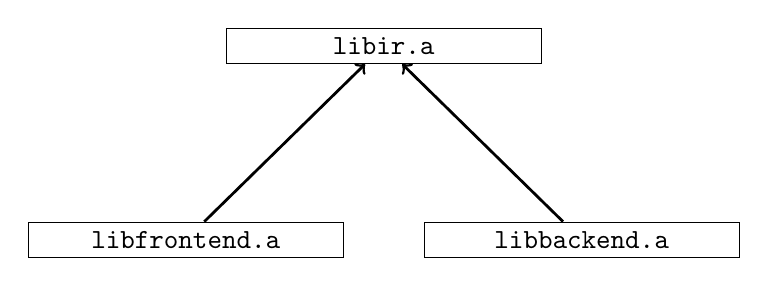
\begin{tikzpicture}
		\node[draw, rectangle, minimum width=4cm, align=center] (ir) {\texttt{libir.a}};
		\node[draw, rectangle, minimum width=4cm, align=center, below left = 2cm and -1.5cm of ir] (frontend) {\texttt{libfrontend.a}};
		\node[draw, rectangle, minimum width=4cm, align=center, below right = 2cm and -1.5cm of ir] (backend) {\texttt{libbackend.a}};

		\draw[->, line width=1pt] (frontend) -- (ir);
		\draw[->, line width=1pt] (backend) -- (ir);
	\end{tikzpicture}
\end{figure}
\subsection{Front-end}
Front-end is implemented in library \texttt{libfrontend.a}. It can be further divided into lexical analyzer, syntax analyzer, semantic analyzer,
and transformation of \emph{abstract syntax tree} (abbr. AST) into
\emph{intermediate representation} (abbr. IR). Each of these parts is described individually in the following paragraphs.

\subsubsection{Lexical, Syntactic and Semantic Analysis}
Lexical analysis is implemented using \texttt{flex}~\cite{flex}, open-source tool for building scanners. Tokens are described in declarative language
by regular expressions and \texttt{flex} automatically constructs C code of the scanner.
The implmentation can be found in \texttt{frontend/c\_lexer.l}.

Syntacitc and semantic analysis is implemented using \texttt{bison}~\cite{bison}, which is made to cooperate with \texttt{flex}. It is tool
for automatic LALR parser generation. The language is described by grammar, which consits of rules that contains non-terminals defined in \texttt{bison} itself
and terminals defined in \texttt{flex} file as tokens. Some tokens are given precedence and associativity, if they represent token for operation.
The grammar in \texttt{bison} is attribute grammar, so it is given a semantic checks and actions. This is used to build AST in a bottom-up parse.
The implementation can be found in \texttt{frontend/c\_parser.y}.

\subsubsection{Context and Symbol Tables}
Language VYPe15 supports nested blocks and every block can have its own variables, which are unreachable outside of the scope of this block. Front-end
therefore needs heirarchical symbol table structure to keep track of these variables and their corresponding blocks. \texttt{Context} serves for this purpose.
It is auxiliary structure that hold global symbol table for functions, stack of symbol tables for variables in functions and nested blocks
and various other contextual information needed during parsing, such as currently parsed function
or currently expected return type. Everytime a parser run into opening of a new block (left curly brace -- \texttt{\{}), it uses \texttt{Context} to create
new symbol table on the stack. Upon running into closing of a block (right curly brace -- \texttt{\}}), parser pops the symbol table from the stack. Symbol tables
popped out from the stack are no longer needed, but they are kept in memory because nodes in AST use pointers to these tables. \texttt{Context} just keep
pointers to all tables it have created because of proper memory deallocation.

Symbol table may contain several symbols, which are stored using C++ STL container \texttt{map}. Symbols are referenced by their name in the map,
which points to their \texttt{Symbol} object. Symbol can be either of type \texttt{VariableSymbol}, \texttt{FunctionSymbol} or \texttt{ManglingLinkSymbol}
(see section XX).

\subsubsection{Abstract Syntax Tree}
Because \texttt{bison} produces bottom-up LALR parser, AST is built from leaf nodes up to the root node. Every node in the tree inherits from the
base class \texttt{ASTNode}. The root node is represented by node \texttt{Program}, which is created implicitly, so parser is trying to build
path from leaf node to the root node. Every node contains pointers either to the child nodes, symbols in the symbol table, textual or numerical
information about the node. AST is transformed directly into IR using interface of \texttt{libir.a} (see section XX) in a depth-first order.

\subsubsection{MINUS: Unary Minus and Plus}
Unary minus and plus represent a problem in parsing, because the same token (\texttt{'-','+'}) has more meanings for two
different operations that have different precedence, associativity and arity. \texttt{bison} offers an easy solution to solve
this problem called \emph{contextual precedence}. We have defined a placeholder tokens \texttt{UNARY\_MINUS} and \texttt{UNARY\_PLUS},
which are not present in the source code and lexer would never return them. They are only given precedence and associativity of
the unary operations they represent. Then we introduced rules in the following form.
\begin{lstlisting}
expr : MINUS expr %prec UNARY_MINUS { ...semantic action... }
     | PLUS expr %prec UNARY_PLUS   { ...semantic action... }
     ;
\end{lstlisting}

It means, whenever one of these rules can be reduced, use precedence and associativity of \texttt{UNARY\_MINUS} respectively \texttt{UNARY\_PLUS}
instead of precedence and associativity of \texttt{MINUS} respectively \texttt{PLUS}, where \texttt{MINUS} and \texttt{PLUS} are just symbolic
names of tokens representing characters \texttt{'-'} and \texttt{'+'}.

\subsubsection{OVERLOAD: Name Mangling}
The extension OVERLOAD allows user to define multiple functions with the same name. The assignment does not specify what should distinguish these functions,
but we have assumed the same functionality as C++ overloading. Functions are distinguished by the amount of parameters or their type. They cannot be distinguished
by their return type. We have solved this problem the similar way how real compilers solve it. We have introduced something what is called \emph{name mangling}.
It is technique that decorates name of the function with additional characters. Those characters are chosen specifically, so they cannot collide with any other
defined function. In our case, it was decoration in the form
\begin{equation*}
	\texttt{\_\$}\langle number\ of\ parameters \rangle\langle parameter\ type\rangle_{1}...\langle parameter\ type\rangle_{n}\texttt{\$}
\end{equation*}

This decoration is appended to every function symbol. Character \texttt{\$} is used because it is not valid character in user defined identifier, therefore
we avoid conflicts. Parameter type is stored in abbreviated form, \texttt{i} for \texttt{int}, \texttt{c} for \texttt{char} and \texttt{s} for \texttt{string}.
If we had function defined as \texttt{void foo(int w, char x, string y, int z)}, the decorated name would be \texttt{foo\_\$4icsi\$}.
Two symbols would be insterted into global symbol table for this function. One \texttt{FunctionSymbol} for name \texttt{foo\_\$4icsi\$} and
one \texttt{ManglingLinkSymbol} for name \texttt{foo}. The \texttt{ManglingLinkSymbol} has two purposes. It contains list of all \texttt{FunctionSymbols} that has the same
original name and it also forbids definition of variable with the same name as function, because \texttt{ManglingLinkSymbol} occupies the original name.

\subsection{IR}
This module of compiler, implemented in \texttt{libir.a}, is completely independent of any other module and can be reused for other compilers. It is slightly
inspired by LLVM framework. It provides a set of instructions in form of hierarchical class structure. Every instruction inherits from class \texttt{Instruction}.
It also implements \emph{control flow graph} (abbr. CFG) management using \texttt{BasicBlock} and \texttt{Function} classes. The interface provides methods
that are able to build whole CFG for list of functions. Instructions operate over objects called \texttt{Values}. \texttt{Value} can be either \texttt{NamedValue},
\texttt{TemporaryValue} or \texttt{ConstantValue}. \texttt{NamedValues} are bound to user-defined variable, those which are actually given name by the user himself.
\texttt{TemporaryValues} are product of the operations and their intermediate results. They are created automatically if any intermediate result needs to be stored
for further evaluation. \texttt{ConstantValue} is templated class that stores constant values in the program.

Similar to LLVM, \texttt{libir} also provides way to write passes. These passes are implemented using \emph{visitor}-like interface. To write a pass, one would
inherit \texttt{IrVisitor} and implement all its \texttt{visit} methods. \texttt{libir} already comes with one pass called \texttt{PrintIrVisitor}, which
is able to print whole CFG in text form.

\subsection{Back-end}
The responsibility of this module is to translate IR code to assembly code. Our target platform is MIPS processor with 1 MB of RAM space. As we have no MIPS device to run the code on, we use simulation program written by Lissom research group. The simulator is capable of running limited MIPS instruction set. In this module we deal with translation of IR instructions to MIPS instructions, simulation of stack, function prologue and epilogue and register allocation.

The module is divided into 4 parts. 
\begin{itemize}
	\item \texttt{Mips} - describes hardware architecture, defines sets of registers used for parameter transfer, regisetrs for evaluation, caller saved and callee saved registers.
	\item \texttt{FunctionContext} - handles function prolog/epilog, mapping of variables at the stack, saving caller saved registers.
	\item \texttt{BlockContext} -- handles register allocation, loading of registers, spilling of variables to stack.
	\item \texttt{AsmGenerator} -- implements \texttt{IrVisitor}, traverses IR instructions and translates it to Mips instructions.
\end{itemize}

\subsubsection{ABI Convention}
In our compiler, we follow the application binary interface known as \textit{O32} \cite{O32}. 
Some restrictions have been put on \textit{\$GP} register, as we use it as the address of first free data in RAM.
Convention for parameter passing and stack cleaning is \texttt{C-decl}.
\subsubsection{Stack}
The MIPS processor has no stack instructions. We have to simulate it using \texttt{ADD}/\texttt{SUB} instructions. As usual, stack grows downward. By the assignment, we are limited to 1 MB of address space. At the beginning of code, we set a O32 dedicated stack pointer \textit{SP} to the address of "\textit{0x10000}" hexadecimal. There is no detection of stack overflow.

Stack manipulation is mostly handled in context of function \texttt{FunctionContext}.

\subsubsection{Frame}
Stack frame represents function context. The function has parameters, local variables and temporary values , return value and return address. The placement of all items is shown on figure TODO. First 4 parameters are transfered through Register \texttt{R4} -- \texttt{R7}, they are copied on stack for future use. Parameters 5 -- $N$ are transfered through stack, so we do not have to copy them to function frame. All local variables(\texttt{NamedValue}) have dedicated place on the stack. Space for temporary values (\texttt{TemporaryValue}) is shared among all temporaries, which exists simultaneously. It is used only if spilling of temporary value occurs or a temporary will be used after function call. In that case the compiler must preserve all temporaries, which haven't been used yet.

\begin{figure}[!h]
	\centering
	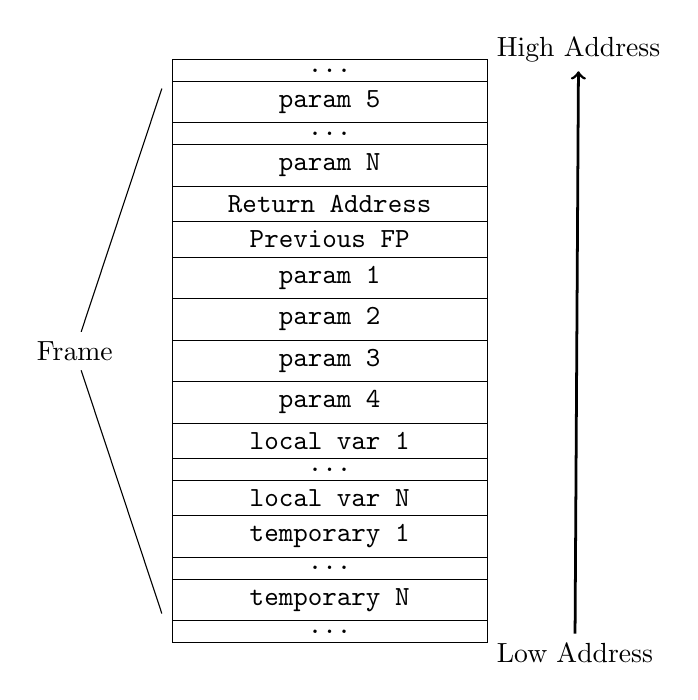
\begin{tikzpicture}
		\matrix[
			matrix of nodes,
			row sep =-\pgflinewidth,
			column sep = -\pgflinewidth,
			nodes={anchor=center, minimum width=4cm, rectangle, draw, font=\ttfamily},
			column 1/.style = {nodes={minimum width=4cm}}
		] (m)
		{
			... \\
			param 5 \\
			... \\
			param N \\
			Return Address \\
			Previous FP \\
			param 1 \\
			param 2 \\
			param 3 \\
			param 4 \\
			local var 1 \\
			... \\
			local var N \\
			temporary 1 \\
			... \\
			temporary N \\
			... \\
		};

		\node[left = 0.5cm of m] (frame) {Frame};
		\node[right = 2cm of m.south] (low) {Low Address};
		\node[right = 2cm of m.north] (high) {High Address};

		\draw[-] ($(m.north -| m.west) + (0cm,-0.5cm)$) -- (frame);
		\draw[-] ($(m.south -| m.west) + (0cm,0.5cm)$) -- (frame);
		\draw[->,line width=1pt] (low) -- (high);
	\end{tikzpicture}
	\caption{Stack Frame}
\end{figure}

\subsubsection{String handling}
Static strings are stored in \textit{data} section of assembly file. First free address is labeled. At the beginning of code, we set \textit{GP} register to this address(label). At runtime, if memory place for dynamic string is needed, a \textit{GP} register points to it. If there is a function call, we store the GP register content to stack and load it back after return from function call. If function returns a string value, we simply create a new dynamic string (using a memory place pointed by \textit{GP}) and copy returned string to this location. This method reduces memory consumption generated by program. Each time a return from function occurs, data memory is returned to state before function call.

Constant literals(\texttt{ConstantValue}) are stored at the beginning of \textit{data} section. There is no redundant literal. Each time a generator requires the address of a constant string, symbol table is searched for a match. If there is no match, new item is added to table. 

There are two embedded functions added to all generated files to support string manipulation. First function copies string returned from a function to local variable. Second function implements C-like strcmp used by relational operators.

\subsubsection{Register allocation}
Register allocation does not use liveness. Every variable mapped in register does have a value, denoting last use. Our implementation uses Least Recently Used(LRU) technique. If there is no more free register and there is a request for free register, a variable must be spilled. Victim is chosen by highest LRU value. As it was written, spilled variable is saved to stack. If variable is constant, it is removed without spilling.

A register allocation is done per basic block. At the beginning of each basic block compiler assumes that all registers are free. Requested variable is given a register and generated a load of variable into register. The load is default, but can be omitted. This is handled by a \texttt{BlockContext} part of backend. 

A temporary value is not needed after used exactly once. If a usage of this value is detected, this value is removed from mapping and discarded permanently.



\subsubsection{Instruction simulation}
In few cases, it is required to simulate IR instructions with a sequence of MIPS instructions. The table bellow shows MIPS instructions simulating IR instructions. There are also string versions of these instructions(they use embedded C-like strcmp), which are not shown.
\begin{center}
	\begin{tabular}{ | c | c | }
		\hline
		IR instruction & MIPS instructions \\
		\hline
		
		$c = (a < b)$  & 
		\begin{tabular}{@{}c@{}}
			SLT c, a, b \\
		\end{tabular}
		\\ \hline
		$c = (a \leq b)$  & 
			\begin{tabular}{@{}c@{}}
				SLT c, a, b \\ 
				XOR tmp, a, b \\
				SLTIU tmp, tmp, 1 \\
				OR c, c, tmp
			\end{tabular}
		\\ \hline
		
		$c = (a > b) $ & 
		\begin{tabular}{@{}c@{}}
			SLT c, b, a \\
		\end{tabular}
		\\ \hline
		
		$c = (a \geq b) $ & 
		\begin{tabular}{@{}c@{}}
			SLT c, b, a \\ 
			XOR tmp, b, a \\
			SLTIU tmp, tmp, 1 \\
			OR c, c, tmp
		\end{tabular}
		\\ \hline
		
		$c = (a == b) $ & 
		\begin{tabular}{@{}c@{}}
			XOR c, a, b \\
			SLTIU c, c, 1 \\
		\end{tabular}
		\\ \hline

		$c = (a != b) $ & 
		\begin{tabular}{@{}c@{}}
			XOR c, a, b \\
			SLTIU c, \$0, c \\
		\end{tabular}
		\\ \hline
		
		$c = (a \&\& b) $ & 
		\begin{tabular}{@{}c@{}}
			SLTIU temp, \$0, a \\
			SLTIU c, \$0, b \\
			AND c, c, temp
		\end{tabular}
		\\ \hline
		
		$c = (a || b) $ & 
		\begin{tabular}{@{}c@{}}
			SLTIU temp, \$0, a \\
			SLTIU c, \$0, b \\
			OR c, c, temp
		\end{tabular}
		\\ \hline
	\end{tabular}
\end{center}

\section{Testing}
Testing is performed on a set of input source codes written in VYPe15, which are compiled into MIPS32 assembly and then they are run
under MIPS32-Lissom simulator. Exit code of the compiler itself and the output of the compiled program are compared with reference
exit code and reference output. We have also build small testing framework to speed up the process of writing and executing tests.
This framework consists of just two bash scripts, \texttt{build\_tests.sh} and \texttt{run.sh}. Both of these scripts can be found in \texttt{testing/}
together with the testsuite.

Every test from a testsuite has its name in form \texttt{test\_name.c}. The reference exit code and output are then stored in files
\texttt{test\_name.ec.ref} and \texttt{test\_name.out.ref}. The output of test after being run is stored in \texttt{test\_name.ec}
and \texttt{test\_name.out}.

The script \texttt{build\_tests.sh} is made to automatically create reference files \texttt{*.ref}. GNU G++ is used for this. However,
language VYPe15 contains few features, which are not present in C++ language. This script therefore modifies tested source code,
so it can be compiled with GNU G++ without changing the semantics of the tested source code.

The script \texttt{run.sh} runs our compiler and then MIPS32-Lissom simulator on the tested source codes in alphabetical order, and informs the user about the result
using colored output if the output is terminal. In case of failed test, also output of \texttt{diff} tool is written to the output.
In order to start \texttt{run.sh}, two environmental variables need to be set.
\begin{itemize}
	\item \texttt{VYPE\_DIR} -- Directory, where compiler named \texttt{vype} is located.
	\item \texttt{MIPS\_DIR} -- Directory, where MIPS32-Lissom simulator is located.
\end{itemize}

\section{Work Division}
The division of work was settled at the beginning of the semester as following.
\begin{itemize}
	\item \textbf{Marek} -- Front-end, IR, writing of tests, documentation
	\item \textbf{Oliver} -- Back-end, writing of tests, documentation
\end{itemize}

We have also held irregular face-to-face meetings, where we discussed our progress and helped each other.
We both did the same amount of work on the compiler and consider this project as a product of both of us.

\clearpage
\bibliographystyle{czechiso}
\begin{flushleft}
	\bibliography{literatura}
\end{flushleft}

\end{document}
